\documentclass[aspectratio=169]{beamer}

% \usetheme{Frankfurt}
\usetheme{Warsaw}

\usecolortheme{seahorse}
\usecolortheme{rose}

\setbeamertemplate{footline}[frame number]
\setbeamertemplate{navigation symbols}[vertical]

\usepackage{verbatim}
\usepackage{fancyvrb}

% ****************************************************************
% Nikhil's defs

% ----------------
% EMPTY BOXES OF VARIOUS WIDTHS, FOR INDENTATION
\newcommand{\hm}{\hspace*{1em}}
\newcommand{\hmm}{\hspace*{2em}}
\newcommand{\hmmm}{\hspace*{3em}}
\newcommand{\hmmmm}{\hspace*{4em}}

\newcommand{\tinytt}{\tiny\tt}
\newcommand{\scripttt}{\scriptsize\tt}

\newcommand{\tick}{\textsc{\char13}}

% ----------------
% SLIDE FONT
\newcommand{\slidefont}{\scriptsize}

% ----------------
% CODE FONT (e.g. {\cf x := 0}).
\newcommand{\cf}{\scriptsize\tt}

% ****************************************************************

\title{A Tour of the RISC-V ISA Formal Specification}

\author{RISC-V Foundation ISA Formal Spec Technical Committee}

\date{
  \begin{tabular}[c]{l}
    
\includegraphics[height=1in]{Figures/Fig_Under_Construction.png}
  \end{tabular}
  \begin{tabular}[c]{l}
    At RISC-V Summit, San Jose \\
    December 12, 2019
  \end{tabular}}

% ****************************************************************
% ****************************************************************
% ****************************************************************

\begin{document}

% ----------------

\begin{frame}
  \titlepage
\end{frame}


% ----------------

\begin{frame}
  \begin{tabular}[c]{l}
    
\includegraphics[height=1.2in]{Figures/Fig_Under_Construction.png}
  \end{tabular}
  \fbox{
  \begin{tabular}[c]{l}
    Dear reader, \emph{Caveat!} we must confess, \\
    This slide deck remains a work in progress, \\
    We suggest, until the target date, please take a recess, \\
    Your cognitive serenity so as not to distress. \\
    \\
    Please come back on December 12, 2019.
  \end{tabular}}
\end{frame}

% ----------------

\begin{frame}
  \frametitle{Location of these slides and additional material}

  These slides are in ``{\tt Slides\_Tutorial.pdf}'' in this GitHub repository:

  \hmm {\tt https://github.com/rsnikhil/RISCV\_ISA\_Spec\_Tour}

  \vspace{3ex}

  The repository also contains ``{\tt Slides\_Installation.pdf}'' which describes

  \hmm Step A that is sufficient for reading the ISA formal spec, and

  \hmm Step B that is needed to create an executable version of the spec.


  \vspace{1ex}

  Please at least perform Step A, which is just to clone the following repository:

  \hmm {\tt https://github.com/rems-project/sail-riscv}

  This is sufficient for most of this tutorial.

\end{frame}

% ----------------

\begin{frame}
  \frametitle{Objectives for this tutorial}

  \slidefont

  \begin{itemize}
    \item \emph{Primary objective}: To give you a basic \emph{reading
      literacy} of the RISC-V ISA Formal Specification, i.e., where
      you are comfortable reading and consulting the formal spec on
      your own on a daily basis.

    \item \emph{Secondary objective}: To show you how to \emph{execute} the
      formal spec on RISC-V binaries, such as standard ISA tests, the
      Compliance Suite, and your own compiled programs.  Typically,
      you'd do this to compare a RISC-V implementation (simulator,
      architectural model, actual hardware implementation) to see if
      the implementation's behavior matches the formal spec
      accurately.

 \end{itemize}

 \emph{Target audience}: Working RISC-V engineers (e.g., CPU
 designers, compiler writers, simulator/emulator writers, ...) who
 consult the spec to clarify understanding of instruction semantics.
 We do not assume any prior experience with formal languages or formal
 methods.

 \vspace{1ex}

 This tutorial may not be suitable for afficionados of formal methods,
 except as an initial familiarization with Sail and the RISC-V formal
 spec.

\end{frame}

% ----------------

\begin{frame}
  \frametitle{Credits}

  \slidefont

  The RISC-V ISA Formal Spec, in the Sail language, was written by:

  \begin{quote}
    Prashanth Mundkur,
    Jon French,
    Brian Campbell,
    Robert Norton-Wright,
    Alasdair Armstrong,
    Thomas Bauereiss,
    Shaked Flur,
    Christopher Pulte,
    Peter Sewell,
    Rishiyur Nikhil
  \end{quote}

  \vspace{4ex}

  The Sail language itself was principally designed and implemented by
  the authors of this paper:

  \vspace{1ex}

  \hfill \begin{minipage}{0.95\textwidth}
    \emph{ISA Semantics for ARMv8-A, RISC-V, and Cheri-MIPS}, \\
    Alasdair Armstrong,
    Thomas Bauereiss,
    Brian Campbell,
    Alastair Reid,
    Kathryn E. Gray,
    Robert M. Norton,
    Prashanth Mundkur,
    Mark Wassell,
    Jon French,
    Christopher Pulte,
    Shaked Flur,
    Ian Stark,
    Neel Krishnaswami,
    Peter Sewell \\
    in \emph{Proc. 46th ACM SIGPLAN Symp. on Principles of Programming
    Languages (POPL), Cascais/Lisbon, Portugal, Jan 13-19, 2019},
    pp. 71:1--71:31.
  \end{minipage}

\end{frame}

% ----------------

\begin{frame}
  \frametitle{Outline}
  \tableofcontents
\end{frame}

% ****************************************************************

\section{Introduction}

% ----------------

\begin{frame}

  \slidefont

  \vfill

  \begin{center}\LARGE
    Introduction
  \end{center}

  \vfill

\end{frame}

% ----------------

\begin{frame}
  \frametitle{Context, briefly}

  \slidefont

  \begin{block}{What is it?}
    \begin{itemize}

      \item The formal spec of the RISC-V ISA is intended to be the
          \emph{definitive} reference for RISC-V instructions:
        \begin{itemize}\slidefont
          \item Encoding
          \item Execution semantics (what executing each instruction is supposed to do)
        \end{itemize}
        More authoritative than the English prose spec (complete, precise, unambiguous).

      \item Excutable: can be run as a simulator executing RISC-V
        binaries, providing definitive execution behaviors

      \item Readable and usable by, and useful to, ordinary mortals who don't do formal stuff for a living.
        \begin{itemize}\slidefont
          \item Casual reading, as a reference guide to RISC-V instructions.
          \item Executable ``golden reference model'' to check implementation correctness.
        \end{itemize}

      \item For those who \emph{do} formal stuff for a living, usable
        with formal tools for proofs of correctness of compilers, CPU
        implementations, automatic generation of tests, test coverage,
        etc.
    \end{itemize}
  \end{block}

\end{frame}

% ----------------

\begin{frame}
  \frametitle{Downloading and Installing}

  Although the slides in this deck are self-contained, containing code
  fragments, we recommend that, in parallel, you view the actual code
  from the repository in a text viewer or editor.  The fragments here
  are excerpts, contain elisions, and cannot show their larger
  context.

  \vspace{1ex}

  {\footnotesize \emph{Each code fragment in this deck shows the file from which it is taken.}}

  \vspace{1ex}

  \begin{block}{Downloading and Installing}
    Please see the separate slide deck {\tt Slides\_Installation.pdf}
    for instructions on how to download the spec, and optionally to
    build an executable version of the spec.
  \end{block}

\end{frame}


% ****************************************************************

\section{Reading the ISA to understand semantics of each RISC-V instruction}

% ----------------

\begin{frame}

  \slidefont

  \vfill

  \begin{center}\LARGE
    Reading the ISA to understand semantics of each RISC-V instruction
  \end{center}

  \vfill

\end{frame}

% ================================================================

\subsection{Preliminaries; Registers and values; ``Scattered'' organization of instruction specs}

% ----------------

\begin{frame}
  \scriptsize

  \begin{block}{About Sail, and the RISC-V ISA Formal Spec written in Sail}
    \begin{itemize}

      \item The RISC-V ISA Formal Spec is written in the language
        Sail, which is a DSL (Domain-Specific Language) designed for
        purpose, i.e., for writing ISA specs.

      \item Sail has been used to describe ISAs for RISC-V, ARMv8
        (complete spec!), MIPS, parts of x86 and IBM POWER, and more.

      \item The Sail manual can be found in the main Sail repository \\
        \hmm {\tt https://github.com/rems-project/sail}

      \item In this tutorial we won't study Sail separately; we'll
        jump into studying the RISC-V Spec written in Sail, explaining
        the Sail notation as we go along.

      \item The RISC-V spec in Sail has its own repository: \\
        \hmm {\tt https://github.com/rems-project/sail-riscv} \\
        We will be studying the code in the {\tt model/} directory.

    \end{itemize}
  \end{block}

\end{frame}

% ----------------

\begin{frame}[fragile]
  \frametitle{A first taste of the semantics}

  \scriptsize

  \begin{Verbatim}[frame=single, label = File riscv\_insts\_base.sail]
function clause execute (RTYPE(rs2, rs1, rd, op)) = {
  let rs1_val = X(rs1);
  let rs2_val = X(rs2);
  let result : xlenbits = match op {
    RISCV_ADD  => rs1_val + rs2_val,
    RISCV_SLL  => if   sizeof(xlen) == 32
                  then rs1_val << (rs2_val[4..0])
                  else rs1_val << (rs2_val[5..0]),
    ... };
  X(rd) = result;
  RETIRE_SUCCESS
}
  \end{Verbatim}

  \begin{itemize}
  \item
    The semantics of each instruction is given by an ``{\cf execute}''
    instruction, a fragment of which is shown above.

  \item
    The function argument says that it is an ``R-format'' instruction
    containing source register fields rs1 and rs2, destination
    register field rd, and an ``op'' sub-opcode identifying the
    specific operation within the group of ``R-format'' instructions.

  \item
    It shows reading the two source registers rs1 and rs2, performing
    the operation specified by ``op'', and writing the result to
    register rd (here showing the ADD and SLL sub-opcodes).
  \end{itemize}

\end{frame}

% ----------------

\begin{frame}[fragile]
  \frametitle{Spec source files (there are a lot of them!)}

  \tiny
  \begin{Verbatim}[frame=single]
--12:50:52--Dell-mation: ~/git_clones/sail-riscv/model
$ ls
main.sail                      riscv_insts_aext.sail    riscv_platform.sail            riscv_termination_duo.sail
prelude_mapping.sail           riscv_insts_base.sail    riscv_pmp_control.sail         riscv_termination_rv32.sail
prelude_mem_metadata.sail      riscv_insts_begin.sail   riscv_pmp_regs.sail            riscv_termination_rv64.sail
prelude_mem.sail               riscv_insts_cext.sail    riscv_pte.sail                 riscv_types_ext.sail
prelude.sail                   riscv_insts_end.sail     riscv_ptw.sail                 riscv_types.sail
README.md                      riscv_insts_mext.sail    riscv_regs.sail                riscv_vmem_common.sail
riscv_addr_checks_common.sail  riscv_insts_next.sail    riscv_reg_type.sail            riscv_vmem_rv32.sail
riscv_addr_checks.sail         riscv_insts_rmem.sail    riscv_step_common.sail         riscv_vmem_rv64.sail
riscv_analysis.sail            riscv_insts_zicsr.sail   riscv_step_ext.sail            riscv_vmem_sv32.sail
riscv_csr_ext.sail             riscv_jalr_rmem.sail     riscv_step_rvfi.sail           riscv_vmem_sv39.sail
riscv_csr_map.sail             riscv_jalr_seq.sail      riscv_step.sail                riscv_vmem_sv48.sail
riscv_decode_ext.sail          riscv_mem.sail           riscv_sync_exception.sail      riscv_vmem_tlb.sail
riscv_duopod.sail              riscv_misa_ext.sail      riscv_sys_control.sail         riscv_vmem_types.sail
riscv_ext_regs.sail            riscv_next_control.sail  riscv_sys_exceptions.sail      riscv_xlen32.sail
riscv_fetch_rvfi.sail          riscv_next_regs.sail     riscv_sys_regs.sail            riscv_xlen64.sail
riscv_fetch.sail               riscv_pc_access.sail     riscv_termination_common.sail  rvfi_dii.sail
  \end{Verbatim}

  \slidefont

  \begin{minipage}{\textwidth}
    Sail does not have a package/module structure--the full Sail
    program is just the concatenation of the source files.

    \vspace{1ex}

    We organize them into files according to our convenience.

    \vspace{1ex}

    In this tutorial we will look at excerpts of some of these files.
  \end{minipage}

\end{frame}

% ----------------

\begin{frame}[fragile]
  \frametitle{A word about types and type-checking}

  
  \begin{itemize}\slidefont

    \item Sail is a strongly-typed language, and does its
      type-checking statically (i.e., on the source code, without
      running the code).

    \item Many types are familiar from other languages (particularly
      functional programming languages): vectors, structs, algebraic
      types/tagged unions, ...

    \item Perhaps the most unfamiliar for many people will be the use
      of numbers as types.

      \begin{itemize}\slidefont

        \item In ISAs (unlike most software programming languages) we
          deal with representations (e.g., bit-vectors) of many
          different sizes, and the precise size is important.

        \item Moreover, sizes of various entities are often related.
          E.g., the shift amount in RV32 (respectively, RV64) should
          be a 5-bit value (respectively, a 6-bit value).  In Sail,
          such relationships can be expressed in types, and are
          type-checked.

      \end{itemize}

    \item Sail also statically keeps track of \emph{effects} (for
      example, does a certain expression read any registers, write any
      registers, ...).  More about this later.

  \end{itemize}

\end{frame}

% ----------------

\begin{frame}[fragile]
  \frametitle{Let's start with some small, easy files}

  \slidefont

  We'd use one of these two files, depending on whether we are considering RV32 or RV64.

  \begin{Verbatim}[frame=single, numbers=left, label = File riscv\_xlen32.sail]
/* Define the XLEN value for the architecture. */

type xlen       : Int = 32
type xlen_bytes : Int = 4
type xlenbits         = bits(xlen)
  \end{Verbatim}

  \begin{Verbatim}[frame=single, numbers=left, label = File riscv\_xlen64.sail]
/* Define the XLEN value for the architecture. */

type xlen       : Int = 64
type xlen_bytes : Int = 8
type xlenbits         = bits(xlen)
  \end{Verbatim}

  \begin{minipage}{\textwidth}
    In lines 3-4, we are defining new \emph{types} that are numeric.

    \vspace{1ex}

    In line 5 we are defining a new type for bit-vectors of size {\cf
      xlen}.  The type {\cf bits(\emph{t})} represents the type of
    bit-vectors of size \emph{t}.  It's parameter \emph{t} must be a
    numeric type (here, we instantiate it as {\cf xlen}).
  \end{minipage}

\end{frame}

% ================================================================

% \subsection{Registers and values}

% ----------------

\begin{frame}[fragile]
  \frametitle{Values in integer registers}

  \slidefont

  \begin{Verbatim}[frame=single, numbers=left, label = File riscv\_reg\_type.sail]
/* default register type */
type regtype = xlenbits

/* default zero register */
let zero_reg : regtype = EXTZ(0x0)
  \end{Verbatim}

  \begin{minipage}{\textwidth}
    In line 2 we're defining the \emph{type} of values in registers;
    it's the same type as {\cf xlenbits}.

    \vspace{1ex}

    In line 5 we're defining a specific \emph{value} of this type,
    using the library function {\cf EXTZ} to zero-extend the constant
    0x0 to the appropriate length.  Because of strong type-checking
    (including some amount of type inference), Sail knows exactly how
    much extension is needed.

    \vspace{1ex}

    Note: the keyword {\cf type} introduces a type definition, the
    keyword {\cf let} introduces a value definition.
  \end{minipage}

\end{frame}

% ----------------

\begin{frame}[fragile]
  \frametitle{Integer registers}

  \slidefont

  \begin{Verbatim}[frame=single, numbers=left, label = File riscv\_regs.sail]
register PC       : xlenbits

register x1  : regtype
register x2  : regtype
...
register x31 : regtype
  \end{Verbatim}

  \begin{minipage}{\textwidth}
    In line 1 with keyword {\cf register} we declare {\cf PC} to be a
    register, and we specify the type of values it can contain, {\cf
      xlenbits}.  The remaining lines similarly declare registers {\cf
      x1}...{\cf x31}.

    \vspace{1ex}

    (There's no {\cf x0} register because it's a constant 0.)

  \end{minipage}

\end{frame}

% ----------------

\begin{frame}[fragile]
  \frametitle{Reading from integer registers}

  \slidefont

  \begin{Verbatim}[frame=single, numbers=left, label = File riscv\_regs.sail]
val rX : forall 'n, 0 <= 'n < 32. regno('n) -> xlenbits effect {rreg, escape}
function rX r = {
  let v : regtype =
    match r {
      0 => zero_reg,
      1 => x1,
      ...
      31 => x31,
      _  => {assert(false, "invalid register number"); zero_reg}
    };
  regval_from_reg(v)
}
  \end{Verbatim}

  \begin{minipage}{\textwidth}
    This defines a function {\cf rX} that takes a register number {\cf
      r} as argument and returns the value contained in that register.
    Line 1, introduced by the {\cf val} keyword, specifies the
    \emph{type} of the function.  It can be read as:

    \begin{quote}
      For all $n$ in the range 0..31, it takes an argument $n$ that is
      a register number, and returns a value of type {\cf xlenbits}.
      Executing this function can have two possible effects, {\cf
        rreg} (reading a register) and {\cf escape} (abort due to
      illegal register number).
    \end{quote}
  \end{minipage}

\end{frame}

% ----------------

\begin{frame}[fragile]
  \frametitle{Reading from integer registers (contd.)}

  \slidefont

  \begin{Verbatim}[frame=single, numbers=left, label = File riscv\_regs.sail]
val rX : forall 'n, 0 <= 'n < 32. regno('n) -> xlenbits effect {rreg, escape}
function rX r = {
  let v : regtype =
    match r {
      0 => zero_reg,
      1 => x1,
      ...
      31 => x31,
      _  => {assert(false, "invalid register number"); zero_reg}
    };
  regval_from_reg(v)
}
  \end{Verbatim}

  \begin{minipage}{\textwidth}
  Line 2, introduced by the {\cf function} keyword, defines the
  function {\cf rX} itself, with argument {\cf r}.

  \vspace{1ex}

  The {\cf let} binding in line 3 introduces a local variable {\cf v}
  and binds it to the value of the ``pattern-matching'' expression in
  Lines 4-10.  This matches the value {\cf r} with each of the
  subsequent patterns 0, 1, 2, ... 31, returning the value of the
  right-hand side on first match.

  \end{minipage}

\end{frame}

% ----------------

\begin{frame}[fragile]
  \frametitle{Reading from integer registers (contd.)}

  \slidefont

  \begin{Verbatim}[frame=single, numbers=left, label = File riscv\_regs.sail]
val rX : forall 'n, 0 <= 'n < 32. regno('n) -> xlenbits effect {rreg, escape}
function rX r = {
  let v : regtype =
    match r {
      0 => zero_reg,
      1 => x1,
      2 => x2,
      ...
      _  => {assert(false, "invalid register number"); zero_reg}
    };
  regval_from_reg(v)
}
  \end{Verbatim}

  \begin{minipage}{\textwidth}
    The type of {\cf v} is {\cf regtype}, i.e., it is a register, and
    so in Line 11 the {\cf regval\_from\_reg(v)} application reads out
    the register value, of type {\cf xlenbits}.

    \vspace{1ex}

    In Sail, a block is a series of expressions in in braces, and the
    value of the last expression is treated as the value of the whole
    block; here, that is also the result of the function.

    \vspace{1ex}

    Observation: improved type-checking and pattern analysis in the
    Sail compiler should allow us to omit the {\cf assert} statement.
    This, in turn, should allow us to omit the {\cf escape} effect.
  \end{minipage}

\end{frame}

% ----------------

\begin{frame}[fragile]
  \frametitle{Writing integer registers}

  \slidefont

  \begin{Verbatim}[frame=single, numbers=left, label = File riscv\_regs.sail]
val wX : forall 'n, 0 <= 'n < 32. (regno('n), xlenbits) -> unit effect {wreg, escape}
function wX (r, in_v) = {
  let v = regval_into_reg(in_v);
  match r {
    0  => (),
    1  => x1 = v,
    ...
    31 => x31 = v,
    _  => assert(false, "invalid register number")
  };
}
  \end{Verbatim}

  \begin{minipage}{\textwidth}
    This is similar to the {\cf rX} read-function.  The function
    type-declaration in line 1 says it takes two arguments, one a
    register number and the second a value of type {\cf xlenbits}, and
    its result type is {\cf unit} which is like the ``void'' type in
    C, indicating a value of no particular interest, since this is a
    pure side effect.  Its effects include {\cf wreg} (writing a
    register) and {\cf escape}.
  \end{minipage}

\end{frame}

% ----------------

\begin{frame}[fragile]
  \frametitle{Using Sail overloading to simplify notation}

  \slidefont

  \begin{Verbatim}[frame=single, numbers=left, label = File riscv\_regs.sail]
overload X = {..., rX, wX}
  \end{Verbatim}

  \begin{minipage}{\textwidth}
    This allows ``{\cf X(r)}'' to be used to read a register (invoking the function ``{\cf rX()}''), \\
    and ``{\cf X(r)=v}'' to write a register (invoking the function ``{\cf wX()}'').
  \end{minipage}

\end{frame}

% ================================================================

% \subsection{``Scattered'' organization of instruction specs}

% ----------------

\begin{frame}[fragile]
  \frametitle{``Scattered'' organization of instruction specs}

  \slidefont

  In a traditional programming language, we might have:
  \begin{itemize}
  \item A type definition showing all the different variants of
      instructions (opcodes, register fields, immediate fields, ...).

    \item A decode function that describes how to take a 32-bit value
      into into each of the different instruction variants.

    \item An execute function that describes how to execute each variant of instruction.
  \end{itemize}

  \vspace{1ex}

  Traditional instruction set manuals ``scatter'' this same
  information differently---a page (or a few) per instruction variant,
  showing:

  \begin{itemize}
    \item Its fields (opcode, register fields, immediate fields, ...).
    \item How a 32-bit instruction is decoded/encoded.
    \item How it is executed.
  \end{itemize}

  \vspace{1ex}

  Sail supports the latter more traditional, familiar organization.
  For each type of instruction, all its relevant information is
  collected in one place.

\end{frame}

% ----------------

\begin{frame}[fragile]
  \frametitle{Introducing things whose clauses will be scattered}

  \slidefont

  We must first introduce the generic information about entities whose
  individual definition-clauses will given later in scattered fashion;
  specifically, types:

  \begin{Verbatim}[frame=single, numbers=left, label = File riscv\_insts\_begin.sail]
scattered union ast

val encdec : ast <-> bits(32)
scattered mapping encdec

val assembly : ast <-> string
scattered mapping assembly
  \end{Verbatim}

  \begin{minipage}{\textwidth}
    Line 1 introduces the type ``{\cf ast}'' which is a \emph{union}
    of all the different variants of instructions.  Each variant will
    follow later, in a scattered fashion.  Here, ``ast'' stands for
    Abstract Syntax Tree, the decoded view of an instruction.

    \vspace{1ex}

    Line 3 declares the type of the ``{\cf encdec}'' mapping, which is
    a pair of functions converting from a 32-bit value (instruction)
    to is decoded view (ast), and vice versa.

    \vspace{1ex}

    Line 6 declares the type of the ``{\cf assembly}''
    mapping that converts from a string to a decoded instruction and
    vice versa.

    \vspace{1ex}

    The ``{\cf scattered}'' annotation and lines indicate that the
    clauses of each of these entities will follow later, in a
    scattered manner.
  \end{minipage}

\end{frame}

% ----------------

\begin{frame}[fragile]
  \frametitle{Introducing things whose clauses will be scattered (contd.)}

  \slidefont

  \begin{Verbatim}[frame=single, numbers=left, label = File riscv\_insts\_begin.sail]
val execute : ast -> Retired effect {escape, wreg, rreg, rmem, ...}
scattered function execute
  \end{Verbatim}

  \begin{minipage}{\textwidth}
    Line 1 declares the type of the ``{\cf execute}'' function, which
    takes a decoded instruction (ast) and returns a ``{\cf Retired}''
    result which indicates whether it should be counted as a retired
    instruction or not.  It also specifies all the possible effects of
    an instruction, such as aborting (``{\cf escape}''), writing and
    reading registers (``{\cf wreg, rreg}''), reading memory, and so on.

    \vspace{1ex}

    The ``{\cf scattered}'' line indicates that the clauses of this
    function will follow later, in a scattered manner.
  \end{minipage}

\end{frame}

% ================================================================

\subsection{Instruction fields}

% ----------------

\begin{frame}[fragile]
  \frametitle{Type definitions for instruction fields}

  \slidefont

  The top of each page in \emph{The RISC-V Instruction Set Manual
    Volume I: Unprivileged ISA}, Chapter 25 \emph{Instruction Set
    Listings} shows the RISC-V formats:

  \vspace{1ex}

  \begin{center}
    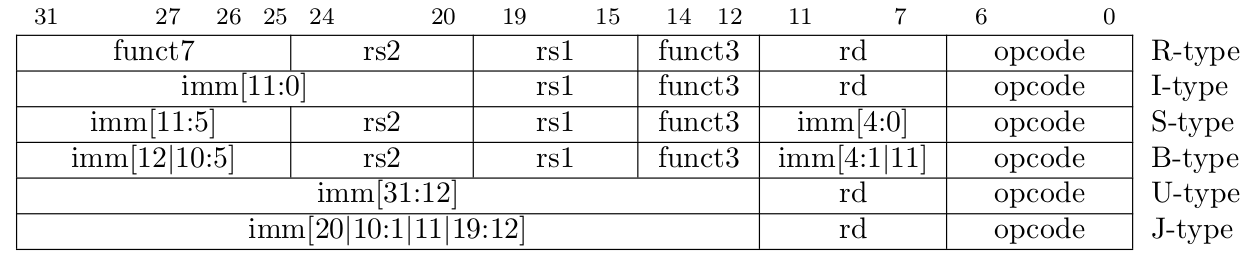
\includegraphics[height=1in]{Figures/Fig_RISCV_formats.png}
  \end{center}

  \vspace{1ex}

  \begin{minipage}{\textwidth}
    \begin{itemize}
    \item The least-significant 7 bits provide a major opcode.
    \item The funct3 and funct7 fields (and sometimes the immediate fields) often
      specify sub-opcodes.
    \item The ``rs1'', ``rs2'' and ``rd'' fields are 5-bit values specifying source and destination registers.
    \item Immediate values are often composed from non-trivial permutation of ``imm'' instruction fields.
    \end{itemize}

  \end{minipage}

\end{frame}

% ----------------

\begin{frame}[fragile]
  \frametitle{Type definitions for instruction fields (contd.)}

  \slidefont

  We declare convenient types for instruction fields.

  \begin{Verbatim}[frame=single, numbers=left, label = File riscv\_types.sail]
type regidx  = bits(5)
type csreg   = bits(12)   /* CSR addressing */
...
type opcode = bits(7)
type imm12  = bits(12)
type imm20  = bits(20)
...
  \end{Verbatim}

  \begin{minipage}{\textwidth}
    These are definitions for register indexes, CSR register
    addresses, major opcodes, and 12-bit and 20-bit immediates.
  \end{minipage}

\end{frame}

% ================================================================

\subsection{Some base instructions}

% ----------------

\begin{frame}[fragile]
  \frametitle{LUI and AUIPC: decoded view}

  \slidefont

  Earlier we declared ``{\cf ast}'' to be a ``{\cf union}'' type,
  i.e., a type with several variants.  We also declared that the
  variants would be provided later in scattered clauses.

  \vspace{1ex}
    
  We now provide one of those clauses, for U-format instructions (LUI and AUIPC):

  \begin{center}
    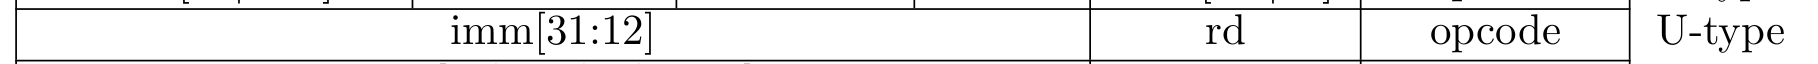
\includegraphics[width=0.8\textwidth]{Figures/Fig_RISCV_U_format.png}
  \end{center}

  \vspace{1ex}
    
  \begin{Verbatim}[frame=single, numbers=left, label = File riscv\_insts\_base.sail]
union clause ast = UTYPE : (bits(20), regidx, uop)
  \end{Verbatim}

  \begin{minipage}{\textwidth}
    This says: one variant of the {\cf ast} type is called {\cf
      UTYPE}.  It contains 3 fields (identified positionally, not with
    keywords) whose types are, respectively, a bit-vector of 20 bits,
    a register index, and a {\cf uop} (which identifies whether it's
    an LUI or AUIPC).

    \vspace{1ex}

    Note: Sail unions are similar to ``algebraic types'' or ``tagged
    unions'' in other programming langauges.  Each value of a tagged
    union carries a way (a ``tag'') by which we can query which
    variant this value encodes.

    \vspace{1ex}

    In Sail, as is common in functional programming languages, values
    of union type are usually analyzed in ``pattern-matching''
    statements, which are like case/switch statements where each
    clause matches a variant of the union.
  \end{minipage}

\end{frame}

% ----------------

\begin{frame}[fragile]
  \frametitle{LUI and AUIPC: Decoding}

  \slidefont

  Earlier, we declared a mapping (a function and its inverse) ``{\cf encdec}'' with this type. \\
  \hmm {\tt val encdec : ast <-> bits(32)} \\
  and further declared that the mapping body would be provided later in scattered clauses.

  \vspace{1ex}
    
  We now provide one such clause, showing how to encode/decode LUI and AUIPC instructions.

  \vspace{1ex}

  \begin{Verbatim}[frame=single, numbers=left, label = File riscv\_insts\_base.sail]
mapping encdec_uop : uop <-> bits(7) = {
  RISCV_LUI   <-> 0b0110111,
  RISCV_AUIPC <-> 0b0010111
}

mapping clause encdec = UTYPE(imm, rd, op)
  <-> imm @ rd @ encdec_uop(op)
  \end{Verbatim}

  \begin{minipage}{\textwidth}
    Lines 1-4 define a new, local mapping between the bit-encodings of the 7-bit
    opcode in a U-format instruction to a value of {\cf uop} type,
    i.e., the symbolic names for the corresponding instructions.

    \vspace{1ex}

    Lines 6-7 add a scattered clause to the ``{\cf encdec}'' mapping.
    The left-hand-side of ``{\cf <->}'' in Line shows the decoded
    view.  The right-hand side shows a bit-concatenation.  The prior
    declarations allow Sail to infer that ``{\cf imm}'', ``{\cf rd}'',
    and ``{\cf encddec\_op(op)}'' are are 20-bit, 5-bit and 7-bit
    fields, respectively, and that the concatenation is a 32-bit
    value,

  \end{minipage}

\end{frame}

% ----------------

\begin{frame}[fragile]
  \frametitle{LUI and AUIPC: execution}

  \slidefont

  Earlier, we declared a function ``{\cf execute}'' with this type. \\
  \hmm {\tt val execute : ast -> Retired effect \{escape, wreg, rreg, rmem, ...\} } \\
  and further declared that the function body would be provided later in scattered clauses.
  Here is the definition of the {\cf Retired} type:

  \vspace{1ex}

  \begin{Verbatim}[frame=single, numbers=left, label = File riscv\_types.sail]
    enum Retired = {RETIRE_SUCCESS, RETIRE_FAIL}
  \end{Verbatim}

  We could have used the ``{\cf bool}'' type for this, but (a) these
  provide more readable names, and (b) this prevents accidental
  confusion of random booleans where an {\cf Retired} value is
  expected.
\end{frame}

% ----------------

\begin{frame}[fragile]
  \frametitle{LUI and AUIPC: execution (contd.)}

  \slidefont

  We now provide one of the clauses for {\cf execute}, for LUI and
  AUIPC instructions.

  \vspace{1ex}

  \begin{Verbatim}[frame=single, numbers=left, label = File riscv\_insts\_base.sail]
function clause execute UTYPE(imm, rd, op) = {
  let off : xlenbits = EXTS(imm @ 0x000);
  let ret : xlenbits = match op {
    RISCV_LUI   => off,
    RISCV_AUIPC => get_arch_pc() + off
  };
  X(rd) = ret;
  RETIRE_SUCCESS
}
  \end{Verbatim}

  \begin{minipage}{\textwidth}
    In Line 1, the argument to the ``{\cf execute}'' function is given
    as a \emph{pattern} ``{\cf UTYPE(imm, rd, op)}''.  Remember {\cf
      execute} can be applied to any value of type {\cf ast}.  The
    pattern here ensures that this clause will only be relevant to
    those {\cf ast} values that are of the {\cf UTYPE} variant.  On a
    successful match, it also binds the names {\cf imm}, {\cf rd} and
    {\cf op} to the three fields of the decoded instruction, so we
    can use these variables in the body of the function.
  \end{minipage}

\end{frame}

% ----------------

\begin{frame}[fragile]
  \frametitle{LUI and AUIPC: execution (contd.)}

  \slidefont

  \begin{Verbatim}[frame=single, numbers=left, label = File riscv\_insts\_base.sail]
function clause execute UTYPE(imm, rd, op) = {
  let off : xlenbits = EXTS(imm @ 0x000);
  let ret : xlenbits = match op {
    RISCV_LUI   => off,
    RISCV_AUIPC => get_arch_pc() + off
  };
  X(rd) = ret;
  RETIRE_SUCCESS
}
  \end{Verbatim}

  \begin{minipage}{\textwidth}
    Strong-typing assures us that {\cf imm} is of type {\cf bits(20)},
    i.e., a bit-vector of length 20.  In Line 2, we concatenate this
    with the 12-bit value 0x000, giving us a 32-bit value.  Then, we
    use {\cf EXTS} to sign-extend it as necessary. This does nothing
    in RV32, since it's already a 32-bit value, and it sign-extends it
    to 64 bits in RV64.  The result is bound to the local variable
    {\cf off} of type {\cf xlenbits}.
  \end{minipage}

\end{frame}

% ----------------

\begin{frame}[fragile]
  \frametitle{LUI and AUIPC: execution (contd.)}

  \slidefont

  \begin{Verbatim}[frame=single, numbers=left, label = File riscv\_insts\_base.sail]
function clause execute UTYPE(imm, rd, op) = {
  let off : xlenbits = EXTS(imm @ 0x000);
  let ret : xlenbits = match op {
    RISCV_LUI   => off,
    RISCV_AUIPC => get_arch_pc() + off
  };
  X(rd) = ret;
  RETIRE_SUCCESS
}
  \end{Verbatim}

  \begin{minipage}{\textwidth}
    Line 3 binds local variable {\cf ret}, of type {\cf xlenbits}, to
    the right-hand side, which is a pattern-matching expression
    examining {\cf op}.  When it matches {\cf RISCV\_LUI}, the value
    is just {\cf off}.  When it matches {\cf RISCV\_AUIPC}, the value
    is added to {\cf get\_arch\_pc()}, which retrieves the value of
    the program counter in the current machine state.

    \vspace{1ex}

    Line 7 assigns this value to register {\cf rd}, using the overloading of {\cf X} we saw earlier.

    \vspace{1ex}

    Finally, Line 8 is the constant expresssion {\cf RETIRE\_SUCCESS}.
    Being the last expression in the block, and the block being the
    body of the function, this is the value returned by the function.
  \end{minipage}

\end{frame}

% ----------------

\begin{frame}[fragile]
  \frametitle{LUI and AUIPC: assembly language parsing and printing}

  \slidefont

  We first define a mapping (function and its inverse) to convert the
  sub-opcode {\cf uop} to a string and back:

  \begin{Verbatim}[frame=single, numbers=left, label = File riscv\_insts\_base.sail]
mapping utype_mnemonic : uop <-> string = {
  RISCV_LUI   <-> "lui",
  RISCV_AUIPC <-> "auipc"
}
  \end{Verbatim}

  Then, we add a scattered clause to our previously introduced {\cf assembly} mapping:

  \begin{Verbatim}[frame=single, numbers=left, label = File riscv\_insts\_base.sail]
mapping clause assembly = UTYPE(imm, rd, op)
  <-> utype_mnemonic(op) ^ spc() ^ reg_name(rd) ^ sep() ^ hex_bits_20(imm)
  \end{Verbatim}

  \begin{minipage}{\textwidth}
    \begin{itemize}
    \item the caret operator concatenates strings; {\cf spc()} and {\cf sep()} return strings for spaces and commas;
    \item {\tt reg\_name(r)} returns the string name for its register-number argument;
    \item {\tt hex\_bits\_20()} returns a string showing a hex printing of a 20-bit value.
    \end{itemize}
  \end{minipage}

\end{frame}

% ----------------

\begin{frame}[fragile]
  \frametitle{Conditional branch instructions: ast clause}

  \slidefont

  Conditional branch instructions include BEQ, BNE, BLT, BGE, BLTU,
  and BGEU: we define symbolic names:

  \vspace{1ex}

  \begin{Verbatim}[frame=single, numbers=left, label = File riscv\_types.sail]
enum bop = {RISCV_BEQ, RISCV_BNE, RISCV_BLT,
            RISCV_BGE, RISCV_BLTU, RISCV_BGEU}    /* branch ops */
  \end{Verbatim}

  Branch instructions are encoded in the B-format:

  \begin{center}
    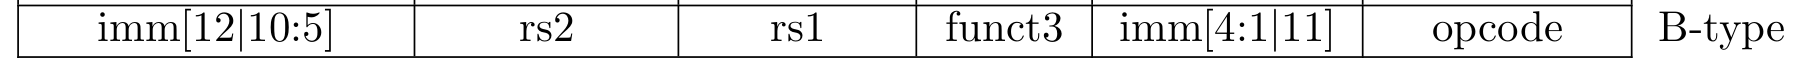
\includegraphics[width=0.8\textwidth]{Figures/Fig_RISCV_B_format.png}
  \end{center}

  Our abstract (decoded) ast view is:

  \vspace{1ex}

  \begin{Verbatim}[frame=single, numbers=left, label = File riscv\_insts\_base.sail]
union clause ast = BTYPE : (bits(13), regidx, regidx, bop)
  \end{Verbatim}

  \begin{minipage}{\textwidth}
    Note:
    \begin{itemize}
    \item The branch offset immediate value is \emph{13 bits}
      composed from 12 bits in the instruction, with 0 appended as
      the least-significant bit.

    \item The 12 bits come from non-contiguous 7-bit and 5-bit fields in the instruction.

    \item Our ast (decoded) view holds the 13-bit offset (computed in the {\cf
      encdec} function to be shown shortly).
    \end{itemize}
  \end{minipage}

\end{frame}

% ----------------

\begin{frame}[fragile]
  \frametitle{Conditional branch instructions: encoding/decoding}

  \slidefont

  We define a mapping converting the 3-bit ``funct3'' field in the instruction to its abstract names:

  \vspace{1ex}

  \begin{Verbatim}[frame=single, numbers=left, label = File riscv\_types.sail]
mapping encdec_bop : bop <-> bits(3) = {
  RISCV_BEQ  <-> 0b000,    RISCV_BNE  <-> 0b001,
  RISCV_BLT  <-> 0b100,    RISCV_BGE  <-> 0b101,
  RISCV_BLTU <-> 0b110,    RISCV_BGEU <-> 0b111
}
  \end{Verbatim}

  Then, we add a scattered clause to the {\cf encdec} mapping:

  \vspace{1ex}

  \begin{Verbatim}[frame=single, numbers=left, label = File riscv\_types.sail]
mapping clause encdec = BTYPE(imm7_6 @ imm5_0 @ imm7_5_0 @ imm5_4_1 @ 0b0, rs2, rs1, op)
<-> imm7_6 : bits(1) @ imm7_5_0 : bits(6)
    @ rs2 @ rs1 @ encdec_bop(op)
    @ imm5_4_1 : bits(4) @ imm5_0 : bits(1)
    @ 0b1100011
  \end{Verbatim}

  \begin{minipage}{\textwidth}
    Observe 13-bit offset is composed by extracting bits from various places in the instruction.
  \end{minipage}

\end{frame}

% ----------------

\begin{frame}[fragile]
  \frametitle{Conditional branch instructions: execution}

  \slidefont

  We add a scattered clause to the {\cf execute} function.  The first part is straightforward:

  \vspace{1ex}

  \begin{Verbatim}[frame=single, numbers=left, label = File riscv\_types.sail]
function clause execute (BTYPE(imm, rs2, rs1, op)) = {
  let rs1_val = X(rs1);
  let rs2_val = X(rs2);
  let taken : bool = match op {
    RISCV_BEQ  => rs1_val == rs2_val,     RISCV_BNE  => rs1_val != rs2_val,
    RISCV_BLT  => rs1_val <_s rs2_val,    RISCV_BGE  => rs1_val >=_s rs2_val,
    RISCV_BLTU => rs1_val <_u rs2_val,    RISCV_BGEU => rs1_val >=_u rs2_val
  };
  let t : xlenbits = PC + EXTS(imm);
  ...
}
  \end{Verbatim}

  \begin{minipage}{\textwidth}
    \begin{itemize}
    \item Line 4 computes ``{\cf taken}'', indicating whether the
      branch is taken or not.  It does a pattern-match on the
      sub-opcode {\cf op}.  Note that BLT and BLTU are supposed to
      interpret their argument as signed and unsigned values,
      respectively.  This is encoded by using different Sail
      pre-defined comparison operators {\cf <\_s} and {\cf <\_u},
      respectively.
    \item Line 9 computes the branch target, adding a sign-extension of the immediate to the PC.
    \end{itemize}
  \end{minipage}


\end{frame}

% ----------------

\begin{frame}[fragile]
  \frametitle{Conditional branch instructions: execution (contd.)}

  \slidefont

  The second part of the {\cf execute} function clause performs
  different actions depending on whether the branch is taken or not:

  \vspace{1ex}

  \begin{Verbatim}[frame=single, numbers=left, label = File riscv\_types.sail]
function clause execute (BTYPE(imm, rs2, rs1, op)) = {
  ...
  if taken then {
    ...
    ...
  } else RETIRE_SUCCESS
}
  \end{Verbatim}

  \begin{minipage}{\textwidth}
    If the branch is not taken, there is no further action and the
    result is {\cf RETIRE\_SUCCESS}.
  \end{minipage}

\end{frame}

% ----------------

\begin{frame}[fragile]
  \frametitle{Conditional branch instructions: execution (contd.)}

  \slidefont

  If the branch would be taken, we first check that the branch target PC is valid.

  \vspace{1ex}

  \begin{Verbatim}[frame=single, numbers=left, label = File riscv\_types.sail]
  if taken then {
    ... <some code elided> ...
        if bit_to_bool(target[1]) & (~ (haveRVC())) then {
          handle_mem_exception(target, E_Fetch_Addr_Align());    RETIRE_FAIL;
        } else {
          set_next_pc(target);    RETIRE_SUCCESS
        }
  \end{Verbatim}

  \begin{minipage}{\textwidth}
    \begin{itemize}
    \item Line 3 checks the requirement that, without the ``C'' ISA
      extension (compressed instructions), the branch target must be
      4-byte aligned, i.e., bit [1] must be 0. {\cf bit\_to\_bool}
      converts a value of {\cf bits(1)} type to {\cf bool} type (we
      could have also used ``{\cf ==1}''). {\cf haveRVC} checks if the
      C extension is active. If the target is not ok, on Line 4 we
      invoke function {\cf handle\_mem\_exception} to perform
      exception actions and return failure.  If the target is ok, Line
      6 assigns it to the next PC and we return success.

    \item Our ``{\cf <some code elided>}'' on Line 2 contains
      additional checks for target validity that may be required by
      any other extensions.
    \end{itemize}
  \end{minipage}


\end{frame}

% ----------------

\begin{frame}[fragile]
  \frametitle{Conditional branch instructions: Assembly language parsing and printing}

  \slidefont

  We first define a mapping (function and its inverse) to convert the
  sub-opcode {\cf bop} to a string and back:

  \begin{Verbatim}[frame=single, numbers=left, label = File riscv\_insts\_base.sail]
mapping btype_mnemonic : bop <-> string = {
  RISCV_BEQ  <-> "beq",     RISCV_BNE  <-> "bne",
  RISCV_BLT  <-> "blt",     RISCV_BGE  <-> "bge",
  RISCV_BLTU <-> "bltu",    RISCV_BGEU <-> "bgeu"
}
  \end{Verbatim}

  Then, we add a scattered clause to our previously introduced {\cf assembly} mapping:

  \begin{Verbatim}[frame=single, numbers=left, label = File riscv\_insts\_base.sail]
mapping clause assembly = BTYPE(imm, rs2, rs1, op)
  <-> btype_mnemonic(op) ^ spc() ^ reg_name(rs1) ^ sep() ^ reg_name(rs2) ^
          sep() ^ hex_bits_13(imm)
  \end{Verbatim}

  \begin{minipage}{\textwidth}
    \begin{itemize}
    \item the caret operator concatenates strings; {\cf spc()} and {\cf sep()} return strings for spaces and commas;
    \item {\tt reg\_name(r)} returns the string name for its register-number argument;
    \item {\tt hex\_bits\_13()} returns a string showing a hex printing of a 13-bit value.
    \end{itemize}
  \end{minipage}

\end{frame}

% ****************************************************************

% ----------------

\begin{frame}[fragile]
  \frametitle{Taking stock ...}

  \slidefont

  The general scheme for adding a new instruction, or new class of instructions, should be clear by now:
  \begin{itemize}
    \item Define an enum and mapping for any sub-opcodes in the class
      (if the class contains more than one instruction)
    \item Augment the ``{\cf ast}'' type by adding a scattered clause to describe this new class
    \item Augment the ``{\cf encdec}'' mapping by adding a scattered clause to describe this new class
    \item Augment the ``{\cf execute}'' function by adding a scattered clause to describe this new class
    \item Augment the ``{\cf assembly}'' mapping by adding a scattered clause to describe this new class
  \end{itemize}

  \vspace{1ex}

  It is a stylistic judgement call whether you define a class with
  sub-opcodes, or just define a separate clause for each instruction
  in the class.  E.g., we could have defined separate ``{\cf ast}'' ,
  ``{\cf encdec}'', ``{\cf execute}'' and ``{\cf assembly}'' clauses
  for BEQ, BNE, BLT, ...

  \vspace{1ex}

  A class with sub-opcodes makes sense when the instructions share
  structure and semantics.  For example, BEQ/BNE/BLT/... differ only
  in the particular comparison operator; using a class with
  sub-opcodes captures this similarity.

  \vspace{1ex}

  \centering
  \emph{For the remaining examples we'll focus on the ``{\cf execute}'' function.}

\end{frame}

% ----------------

\begin{frame}[fragile]
  \frametitle{LOAD instructions: execution}

  \slidefont

  Memory-access instructions involve many more steps, since they can
  involve alignment checks, virtual address-to-physical address
  translation, physical memory protection checks, ordering
  relationships with other memory accesses, and so on.  Many of these
  can trap (raise an exception).

  \vspace{1ex}

  The header of a memory-load instruction:

  \vspace{1ex}

  \begin{Verbatim}[frame=single, numbers=left, label = File riscv\_insts\_base.sail]
function clause execute(LOAD(imm, rs1, rd, is_unsigned, width, aq, rl)) = {
  \end{Verbatim}

  \begin{minipage}{\textwidth}
    The arguments are the
    \begin{itemize}
    \item the immediate, rs1 and rd fields from the instruction;

    \item whether the loaded value is treated as signed or unsigned,
      i.e., whether the loaded value should be sign-extended or
      zero-extended to the width of the destination register;

    \item the width: byte, halfword (2 bytes), word (4 bytes) or double (8 bytes);

    \item the acquire/release semantics for memory ordering.
    \end{itemize}
  \end{minipage}

\end{frame}

% ----------------

\begin{frame}[fragile]
  \frametitle{LOAD instructions: execution (contd.)}

  \slidefont

  The next step is to compute the actual (virtual) address to be accessed:

  \begin{Verbatim}[frame=single, numbers=left, label = File riscv\_insts\_base.sail]
  let offset : xlenbits = EXTS(imm);
  match ext_data_get_addr(rs1, offset, Read(Data), width) {
    Ext_DataAddr_Error(e)  => { ext_handle_data_check_error(e); RETIRE_FAIL },
    Ext_DataAddr_OK(vaddr) =>
        ...
  \end{Verbatim}

  \begin{minipage}{\textwidth}
    After computing the offset by sign-extending the immediate value,
    it invokes the function ``{\cf ext\_data\_get\_addr}'' to perform
    a signed addition to the contents of rs1.  This function is
    defined in ``{\cf riscv\_addr\_checks.sail}''.  By encapsulating
    this addition in a function, we allow future extensibility to new
    ISA extensions that may peform additional checks/transformations
    on the address.

    \vspace{1ex}

    This function can return an error, but in the normal simple case
    without additional ISA extensions it returns ``{\cf
      Ext\_DataAddr\_OK(vaddr)} containing the effective virtual
    address.  We use a {\cf match} expression to distinguish these two
    outcomes.
  \end{minipage}


\end{frame}

% ----------------

\begin{frame}[fragile]
  \frametitle{LOAD instructions: execution (contd.)}

  \slidefont

  Next:

  \begin{Verbatim}[frame=single, numbers=left, label = File riscv\_insts\_base.sail]
      if   check_misaligned(vaddr, width)
      then { handle_mem_exception(vaddr, E_Load_Addr_Align()); RETIRE_FAIL }
      else match translateAddr(vaddr, Read(Data)) {
          ...
  \end{Verbatim}

  \begin{minipage}{\textwidth}
    The function ``{\cf check\_misaligned(vaddr, width)}'' optionally
    checks if the access is aligned for the requested width.  This
    function is defined a little earlier in the file and returns true
    it is misaligned \emph{and if we've configured the model to
      disallow misaligned accesses}.

    \vspace{1ex}

    If ok, it invokes ``{\cf translateAddr(vaddr, Read(Data)}'' to
    optionally translate virtual addresses to physical addresses.
    This function is defined in a collection of files: \\
    \hm {\cf riscv\_vmem\_rv32.sail}, {\cf riscv\_vmem\_sv32.sail} \\
    \hm {\cf riscv\_vmem\_rv64.sail}, {\cf riscv\_vmem\_sv39.sail}, {\cf riscv\_vmem\_sv48.sail} \\
    \hm {\cf riscv\_vmem\_tlb.sail} \\
    different subsets of which are used depending on whether we're
    modeling RV32 or RV64, and the Sv32, Sv39 or Sv48 virtual memory
    schemes.

    \vspace{1ex}

    The function simply returns the address as-is if not running with
    virtual memory.

    \vspace{1ex}

    In the virtual-memory translation functions, you'll notice that
    they also model a TLB (Translation Lookaside Buffer).  This is
    because TLBs are visible in the semantics via the SFENCE.VMA
    instruction.

  \end{minipage}


\end{frame}

% ----------------

\begin{frame}[fragile]
  \frametitle{LOAD instructions: execution (contd.)}

  \slidefont

  Finally:

  \begin{Verbatim}[frame=single, numbers=left, label = File riscv\_insts\_base.sail]
      else match translateAddr(vaddr, Read(Data)) {
        TR_Failure(e, _) => { handle_mem_exception(vaddr, e); RETIRE_FAIL },
        TR_Address(addr, _) =>
          match (width, sizeof(xlen)) {
            (BYTE, _)   =>
               process_load(rd, vaddr, mem_read(Read(Data), addr, 1, aq, rl, false), is_unsigned),
            (HALF, _)   =>
               process_load(rd, vaddr, mem_read(Read(Data), addr, 2, aq, rl, false), is_unsigned),
            (WORD, _)   =>
               process_load(rd, vaddr, mem_read(Read(Data), addr, 4, aq, rl, false), is_unsigned),
            (DOUBLE, 64) =>
               process_load(rd, vaddr, mem_read(Read(Data), addr, 8, aq, rl, false), is_unsigned)
  \end{Verbatim}

  \begin{minipage}{\textwidth}
    If the virtual-to-physical translation was successful, we invoke
    ``{\cf mem\_read}'' to perform the raw memory read, and pass the
    result to ``{\cf process\_load}'' to process the result (which
    could be an exception, e.g, if there is no memory at that
    address).

    \vspace{1ex}

    The first three clauses of the ``{\cf match}'' expression use the
    wildcard pattern ``{\cf \_}'' in the second component, since these
    sizes are valid in RV32 and RV64.  The fourth clause will only
    match when the second component is 64, i.e., it restricts it to
    RV64.

  \end{minipage}


\end{frame}

% ================================================================

\subsection{Exceptions}

% ----------------

\begin{frame}[fragile]
  \frametitle{Exceptions}

  \slidefont

  RISC-V has
  \begin{itemize}
  \item interrupts (asyncnronous exceptions, conceptually ``between'' any two instructions)
  \item traps (synchronous exceptions, due to execution of an instruction)
  \end{itemize}

  \vspace{1ex}

  The different kinds of interrupts:

  \vspace{1ex}

  \begin{Verbatim}[frame=single, numbers=left, label = File riscv\_types.sail]
enum InterruptType = {  I_U_Software,    I_S_Software,    I_M_Software,
                        I_U_Timer,       I_S_Timer,       I_M_Timer,
                        I_U_External,    I_S_External,    I_M_External    }
  \end{Verbatim}

  The file also contains a function to convert bit-encodings to these symbolic names:

  \vspace{1ex}

  \begin{Verbatim}[frame=single, numbers=left, label = File riscv\_types.sail]
val interruptType_to_bits : InterruptType -> bits (8)
function interruptType_to_bits (i) = match (i) {   I_U_Software => 0x00,
                                                   I_S_Software => 0x01,  ... }
  \end{Verbatim}

  Comment: A mapping would be more expressive than a function, but
  since we don't decode interrupts/exceptions, we don't need the inverse
  function.

\end{frame}

% ----------------

\begin{frame}[fragile]
  \frametitle{Exceptions (contd.)}

  \slidefont

  The different kinds of traps, and converting to bits:

  \begin{Verbatim}[frame=single, numbers=left, label = File riscv\_types.sail]
union ExceptionType = { E_Fetch_Addr_Align   : unit,     E_Fetch_Access_Fault : unit,
                        E_Illegal_Instr      : unit,     E_Breakpoint         : unit,
                        E_Load_Addr_Align    : unit,     E_Load_Access_Fault  : unit,
                        E_SAMO_Addr_Align    : unit,     E_SAMO_Access_Fault  : unit,
                        E_U_EnvCall          : unit,     E_S_EnvCall          : unit,
                        E_Reserved_10        : unit,     E_M_EnvCall          : unit,
                        E_Fetch_Page_Fault   : unit,     E_Load_Page_Fault    : unit,
                        E_Reserved_14        : unit,     E_SAMO_Page_Fault    : unit }

val exceptionType_to_bits : ExceptionType -> exc_code
function exceptionType_to_bits(e) = match (e) { E_Fetch_Addr_Align()   => 0x00,
                                                E_Fetch_Access_Fault() => 0x01, ...}
  \end{Verbatim}

  \begin{minipage}{\textwidth}
    Comment: I think this could also have been written as an
    enum.  The ``{\cf unit}'' type is like {\cf void}, so these union
    variants don't contain any interesting data with each tag.
  \end{minipage}

\end{frame}

% ----------------

\begin{frame}[fragile]
  \frametitle{Exceptions (contd.)}

  \slidefont

  Some traps may carry additional information.  In Sail (and OCaml),
  optional information is usually expressed using the ``{\cf option}''
  predefined type:

  \begin{Verbatim}[frame=single, numbers=left, label = predefined]
union option ('a : Type) = { Some : 'a,
                             None : unit }
  \end{Verbatim}

  i.e., the ``{\cf Some}'' variant carries some additional information
  (generic/polymorphic type {\cf 'a}), and the``{\cf None}'' variant
  carries no additional information.

  \vspace{1ex}

  \begin{Verbatim}[frame=single, numbers=left, label = File riscv\_sync\_exception.sail]
struct sync_exception = { trap    : ExceptionType,
                          excinfo : option(xlenbits),
                          ext     : option(ext_exception)   /* for extensions */ }
  \end{Verbatim}

  \begin{minipage}{\textwidth}
    The ``{\cf trap}'' field is necessary information.  The other two
    fields carry optional information, for standard traps (such as an
    address that provoked a trap), and also for future standard or
    non-standard ISA extensions.
  \end{minipage}

\end{frame}

% ----------------

\begin{frame}[fragile]
  \frametitle{Handling certain exceptions}

  \slidefont

  The ``{\cf handle\_mem\_exception}'' action function we saw earlier
  in conditional branches with illegal branch targets is:

  \vspace{1ex}

  \begin{Verbatim}[frame=single, numbers=left, label = File riscv\_sys\_control.sail]
function handle_mem_exception(addr : xlenbits, e : ExceptionType) -> unit = {
  let t : sync_exception = struct { trap    = e,
                                    excinfo = Some(addr),
                                    ext     = None() } in
  set_next_pc(exception_handler(cur_privilege, CTL_TRAP(t), PC))
}
  \end{Verbatim}

  \begin{minipage}{\textwidth}
    Lines 1-3 construct a ``{\cf sync\_exception}'' value, filling in
    the address as optional exception info, and binds it to the local
    variable ``{\cf t}''.

    \vspace{1ex}

    In Line 4 we invoke a more general ``{\cf exception\_handler}'' (next slide).
  \end{minipage}

\end{frame}

% ----------------

\begin{frame}[fragile]
  \frametitle{Handling exceptions (contd.)}

  \slidefont

  \begin{Verbatim}[frame=single, numbers=left, label = File riscv\_sys\_control.sail]
function exception_handler(cur_priv : Privilege, ctl : ctl_result,
                           pc: xlenbits) -> xlenbits = {
  match (cur_priv, ctl) {
    (_, CTL_TRAP(e)) => {
      let del_priv = exception_delegatee(e.trap, cur_priv);
      ...
      trap_handler(del_priv, false, exceptionType_to_bits(e.trap), pc, e.excinfo, e.ext)
    },
    (_, CTL_MRET())  => { ... }
    (_, CTL_SRET())  => { ... }
    (_, CTL_URET())  => { ... } }
  \end{Verbatim}

  \begin{minipage}{\textwidth}
    Line 5 checks if the current trap, at the current privilege level,
    is being delegated to be handled at a different privilege level
    (returning that, or the current, privilege level).

    \vspace{1ex}

    Line 7 invokes an even more general trap handler (next slide).

    \vspace{1ex}

    Lines 9-11 handle exception returns from the Machine, Supervisor
    and User privilege levels, respectively.
  \end{minipage}

\end{frame}

% ----------------

\begin{frame}[fragile]
  \frametitle{Handling exceptions (contd.)}

  \slidefont

  \begin{Verbatim}[frame=single, numbers=left, label = File riscv\_sys\_control.sail]
function trap_handler(del_priv : Privilege, intr : bool, c : exc_code,
                      pc : xlenbits, info : option(xlenbits), ext : option(ext_exception))
                     -> xlenbits = {
  cancel_reservation();    /* for LR/SC */
  match (del_priv) {
    Machine => { mcause->IsInterrupt() = bool_to_bits(intr);
                 mcause->Cause()       = EXTZ(c);
                 mstatus->MPIE()       = mstatus.MIE();    mstatus->MIE() = 0b0;
                 mstatus->MPP()        = privLevel_to_bits(cur_privilege);
                 mtval                 = tval(info);       mepc           = pc;
                 cur_privilege         = del_priv;
                 prepare_trap_vector(del_priv, mcause) },
    Supervisor => { ... }
    User => { ... }
  \end{Verbatim}

  \begin{minipage}{\textwidth}
    This is an intricate but otherwise unremarkable assignment of certain values to certain CSRs.

    \vspace{1ex}

    Line 15 invokes ``{\cf prepare\_trap\_vector}'' (in file ``{\cf
      riscv\_sys\_extensions.sail}'') which returns the PC that is in
    ``{\cf mtvec}'', ``{\cf stvec}'', or ``{\cf utvec}'', as appropriate.

  \end{minipage}

\end{frame}

% ----------------

\begin{frame}

  \slidefont

  \vfill

  \begin{center}\LARGE
    Executing complete programs
  \end{center}

  \vfill

\end{frame}

% ----------------

\begin{frame}[fragile]
  \frametitle{Executing complete programs}

  \slidefont

  \begin{itemize}
  \item So far, we've only talked about the decode and execute
    function for individual instructions.  We've said nothing about
    how and when these get invoked, nor about how instructions are
    fetched.

  \item This separation is deliberate.  We may wish to build several
    different processor models: pipelined, superscalar, multi-hart,
    and so on.  Each of these would be a different top-level system,
    with its own system-level semantics, but they can all share the
    individual instruction semantics discussed so far.

  \item In the slides that follow, we'll sketch one such encapsulating
    model, which is used in the default simulators built from the
    model.  This model, shown in files ``{\cf main.sail}'' and ``{\cf
      riscv\_step.sail}'' implement a simple, sequential, unpipelined,
    one-instruction-at-a-time fetch-execute loop ().
  \end{itemize}

\end{frame}

% ----------------

\begin{frame}[fragile]
  \frametitle{Executing complete programs (contd.)}

  \slidefont

  The top-level function initializes the PC, initializes the model as
  a whole (including certain CSRs and registers), and performs the
  fetch-execute loop:

  \vspace{1ex}

  \begin{Verbatim}[frame=single, numbers=left, label = File main.sail]
function main () : unit -> unit = {
  PC = sail_zero_extend(0x1000, sizeof(xlen));
  init_model();
  loop()
}
  \end{Verbatim}

  The loop, in turn, repeatedly performs a fetch-execute step:

  \vspace{1ex}

  \begin{Verbatim}[frame=single, numbers=left, label = File riscv\_step.sail]
function loop () : unit -> unit = {
  while (...) do {
    let stepped = step(step_no);
    ...
  }
}
  \end{Verbatim}

\end{frame}

% ----------------

\begin{frame}[fragile]
  \frametitle{Executing complete programs (contd.)}

  \slidefont

  \begin{Verbatim}[frame=single, numbers=left, label = File riscv\_step.sail]
function step(step_no : int) -> bool = {
  let (retired, stepped) : (Retired, bool) =
    match dispatchInterrupt(cur_privilege) {
      Some(intr, priv) => { handle_interrupt(intr, priv); (RETIRE_FAIL, false) },
      None() => {
        let f : FetchResult = ext_fetch_hook(fetch());
        match f {
          F_RVC(h) => { let ast = decodeCompressed(h);
                        (execute(ext_post_decode_hook(ast)), true) ... }
          F_Base(w) => { let ast = decode(w);
                         nextPC = PC + 4;
                         (execute(ext_post_decode_hook(ast)), true) ... }
}
  \end{Verbatim}

  \begin{minipage}{\textwidth}
    \begin{itemize}
    \item The step first checks for interrupts and handles it if there is one.
    \item If not, it fetches and instruction and decides whether its
      an RVC (compressed) instruction or a base instruction.
    \item In each case, it decodes it and executes it.
    \end{itemize}
  \end{minipage}
\end{frame}

% ****************************************************************

% ----------------

\begin{frame}[fragile]
  \frametitle{Taking stock ...}

  \slidefont

  By this time we hope you're getting the hang of reading the Sail
  code that expresses the semantics of RISC-V instructions.  Some
  observations:
  
  \begin{itemize}
    \item In many senses, Sail is ``just another'' programming
      language.  Many of its notations and features are taken from or
      inspired by the functional programming language OCaml (which, in
      turn, was inspired by SML).

    \item Expressing the semantics of RISC-V instructions is an
      exercise in coding in this programming language.

    \item Features like numeric types with type-checking, scattered
      definitions, mappings, bit-vectors with type-encoded lengths all
      make it into a DSL (Domain Specific Language) for expressing
      ISAs.

    \item Sail's simple, clean, semantics make it suitable for
      connecting to well-known formal-method tools (such as Coq,
      Isabelle, HOL4).

  \end{itemize}

\end{frame}

% ----------------

\begin{frame}[fragile]
  % \frametitle{Overview of spec module dependencies}

  \slidefont

  \begin{tabular}[c]{l}
    
\includegraphics[height=3in]{Figures/riscvspecdeps.png}
  \end{tabular}
  \hmmm
  \begin{tabular}[c]{l}
    Overview of module dependencies in the \\
    Sail RISC-V spec. \\
    \\
    \tiny (Original: {\tt doc/figs/riscvspecdeps.svg} in repo \\
    \hm\tiny\tt https://github.com/rems-project/sail-riscv )
  \end{tabular}

\end{frame}

% ****************************************************************

\section{Executing ISA and Compliance tests}

% ----------------

\begin{frame}

  \slidefont

  \vfill

  \begin{center}\LARGE
    Executing ISA Tests
  \end{center}

  \vfill

\end{frame}

% ================================================================

\subsection{Executing standard RISC-V ISA tests}

% ----------------

\begin{frame}
  \frametitle{Executing standard RISC-V ISA tests}

  {\scripttt sail-riscv/test/riscv-tests/} has a full suite of
  pre-compiled standard RISC-V ISA tests.  Each has an ELF file
  (RISC-V binary) and a disassembly (text file) of the test:

  \begin{block}{Example of ISA test ELF file and disassembly text file}
    \slidefont
    \begin{tabular}{ll}
      \tt \$ ls -1 test/riscv-tests/rv64ui-p-add* \hmm & \\
      \tt test/riscv-tests/rv64ui-p-add.elf            & RISC-V executable \\
      \tt test/riscv-tests/rv64ui-p-add.dump           & Disassembly text file \\
      \tt test/riscv-tests/rv64ui-p-addi.elf           & \\
      \tt test/riscv-tests/rv64ui-p-addi.dump          & \\
      \tt test/riscv-tests/rv64ui-p-addiw.elf          & \\
      \tt test/riscv-tests/rv64ui-p-addiw.dump         & \\
      \tt test/riscv-tests/rv64ui-p-addw.elf           & \\
      \tt test/riscv-tests/rv64ui-p-addw.dump          &
    \end{tabular}
  \end{block}

\end{frame}

% ----------------

\begin{frame}
  \frametitle{Executing standard RISC-V ISA tests (contd.)}

  Using the C-based simulator:

  \begin{block}{Example: executing the {\scripttt rv64ui-p-add} standard ISA test}
    \tiny\tt
    \begin{tabular}{l}
      \$ ./c\_emulator/riscv\_sim\_RV64  rv64ui-p-add \\
      ... \\
      tohost located at 0x80001000 \\
      ... \\
      Running file test/riscv-tests/rv64ui-p-add.elf. \\
      ELF Entry @ 0x80000000 \\
      ... \\\relax
      [0] [M]: 0x0000000000001000 (0x00000297) auipc t0, 0 \\
      ... \\\relax
      [1] [M]: 0x0000000000001004 (0x02028593) addi a1, t0, 32 \\
      ... \\\relax
      [2] [M]: 0x0000000000001008 (0xF1402573) csrrs a0, zero, mhartid \\
      ... \\\relax
      [477] [M]: 0x0000000080000044 (0xFC3F2023) sw gp, 4032(t5) \\
      ... \\
      SUCCESS
    \end{tabular}
  \end{block}

  During execution of the RISC-V binary, it prints out a trace of instructions executed.

\end{frame}

% ----------------

\begin{frame}
  \frametitle{Executing standard RISC-V ISA tests (contd.)}

  Using the OCaml-based simulator:

  \begin{block}{Example: executing the {\scripttt rv64ui-p-add} standard ISA test}

    \tiny\tt
    \begin{tabular}{l}
      \$ ./ocaml\_emulator/riscv\_ocaml\_sim\_RV64  rv64ui-p-add \\
      Sail/RISC-V: running ELF file test/riscv-tests/rv64ui-p-add.elf \\
      ... \\\relax
      [0] [M]: 0x0000000000001000 (0x00000297) auipc t0, 0 \\
      ... \\\relax
      [1] [M]: 0x0000000000001004 (0x02028593) addi a1, t0, 32 \\
      ... \\\relax
      [2] [M]: 0x0000000000001008 (0xF1402573) csrrs a0, zero, mhartid \\
      ... \\\relax
      [477] [M]: 0x0000000080000044 (0xFC3F2023) sw gp, 4032(t5) \\
      ... \\
      SUCCESS
    \end{tabular}
  \end{block}

\end{frame}

% ================================================================

\subsection{Executing Compliance tests}

% ----------------

\begin{frame}

  \slidefont

  \vfill

  \begin{center}\LARGE
    Executing Compliance Tests
  \end{center}

  \vfill

\end{frame}

% ----------------

\begin{frame}
  \frametitle{Executing Compliance tests}

  ... to be written ...
\end{frame}

% ****************************************************************

\section{Extra material}

% ----------------

\begin{frame}

  \slidefont

  \vfill

  \begin{center}\LARGE
    Extra Material
  \end{center}

  \vfill

\end{frame}

% ================================================================

\subsection{A word about concurrency}

% ----------------

\begin{frame}
  \frametitle{A word about concurrency}

  \slidefont

  \begin{itemize}

  \item
    In this introductory tutorial we have deliberately stayed away
    from questions of concurrency, which is a more advanced topic.

  \item
    Each instruction semantics can be regarded as a small sequential
    thread performing that instruction's semantics.  There are various
    ``events'' during this thread's progress: reading a register,
    computing an effective address (for memory accesses), requesting
    memory, getting a response from memory, writing a register, etc.

  \item
    In our simple one-instruction-at-a-time fetch-execute loop model
    shown earlier, these threads are simply concatenated into an
    overall single sequential thread.

  \item
    A parallel model can overlap these threads: a pipeline model may
    launch the next instruction's thread before the current one has
    finished; a superscalar model may launch two or more of these
    threads together; an out-of-order model may have many of these
    threads running concurrently; and so on.

  \item
    Such a parallel model can capture all the complexities of modern,
    sophisticated, high-performance, parallel CPU implementations. In
    particular, such a model can exercise interesting interactions
    with weak memory models.

  \end{itemize}

\end{frame}

% ----------------

\begin{frame}
  \frametitle{Relationship with the official RISC-V Memory Model}

  \slidefont

  \begin{itemize}
  \item
    RISC-V's Weak Memory Model was developed by a separate RISC-V
    Foundation Technical Group, chaired by Dan Lustig of NVidia.

  \item 
    One of their formalizations was indeed using this Sail model.  As
    mentioned in the previous slide, this uses a concurrent
    fetch-execute model where multiple instructions may be in flight
    concurrently, with concurrent interactions with the weak memory
    model.

  \item
    (These details should be covered in another, more advanced tutorial.)

  \end{itemize}

\end{frame}

% ================================================================

\begin{frame}
  \frametitle{Status and Plans}

  \slidefont

  \begin{itemize}
  \item
    The RISC-V Foundation set up a Technical Group (TG) in 2017 to
    develop a Formal Specifcation for the RISC-V ISA, which will
    become the \emph{definitive} specification of the ISA.  There are
    currently 110 members, of which 15-20 were regular attendees of
    weekly con-calls.

  \item 
    The group encompassed 6 different, parallel, efforts, including
    this one in Sail.  In March/April 2019 we put out a public review
    of these efforts.  Based on the feedback and discussions in the
    TG, we decided to move forward with Sail as the main canonical
    spec. It is also the most advanced of the 6 efforts in terms of
    feature coverage and modeling concurrency.  The other 5 efforts
    continue, and over time could achieve peer status with this Sail
    spec.

  \item
    The immediate priority is to clean up, polish, document, and make
    it easily accessible to the community (of which this tutorial is a
    part).

  \end{itemize}

\end{frame}

% ----------------

\begin{frame}
  \frametitle{Sail: the larger picture}

  \slidefont

  In addition to RISC-V, Sail has also been used to specify other
  ISAs.  In addition to the so-called ``C-based'' back-end we've seen
  in this tutorial, it has more back-ends to create an OCaml-based
  simulator, and to connect to various formal environments such as
  Coq, Isabelle, HOL4, etc.

  \vspace{2ex}

  Recommended reference with more details:
  
  \vspace{2ex}

  \hfill \begin{minipage}{0.95\textwidth}
    \emph{ISA Semantics for ARMv8-A, RISC-V, and Cheri-MIPS}, \\
    Alasdair Armstrong,
    Thomas Bauereiss,
    Brian Campbell,
    Alastair Reid,
    Kathryn E. Gray,
    Robert M. Norton,
    Prashanth Mundkur,
    Mark Wassell,
    Jon French,
    Christopher Pulte,
    Shaked Flur,
    Ian Stark,
    Neel Krishnaswami,
    Peter Sewell \\
    in \emph{Proc. 46th ACM SIGPLAN Symp. on Principles of Programming
    Languages (POPL), Cascais/Lisbon, Portugal, Jan 13-19, 2019},
    pp. 71:1--71:31.
  \end{minipage}

  \vspace{2ex}

  See also the figure on the next slide.
\end{frame}

% ----------------

\begin{frame}
  \frametitle{Sail: the larger picture (contd.)}

  \begin{figure}[htbp]
    \centerline{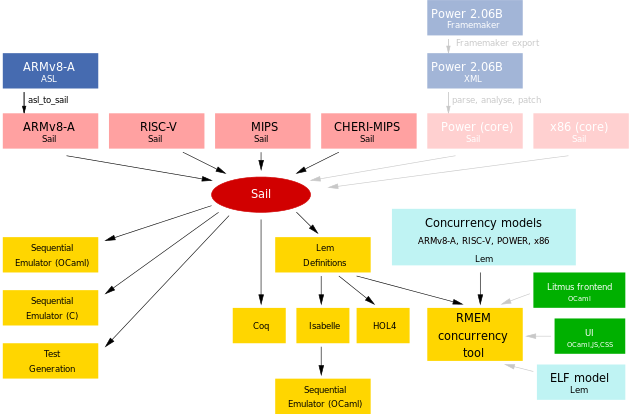
\includegraphics[height=2.3in]{Figures/overview-sail.png}}
    {\scriptsize (from: {\tt https://github.com/rems-project/sail})}
  \end{figure}

\end{frame}

% ----------------

\begin{frame}
  \frametitle{Adding new ISA Extensions}

  ... to be written ...
\end{frame}

% ----------------

\begin{frame}
  \frametitle{How people use ISA formal specs}

  \slidefont

  People are already using and will use the ISA formal spec in various ways.

  \begin{itemize}
    \item As a reference to clarify the intended semantics of each type of instruction.

    \item As a ``golden reference model'' against which to compare
      other implementations (simulation to hardware designs) for
      correctness.  Specific examples include official Compiance
      Tests, and Tandem Verification.

    \item In a tool to generate ISA tests automatically.

    \item In a tool to measure instruction coverage automatically.

    \item In a tool to formally prove a separately-written
      implementation correct, by directly correlating the ISA formal
      semantics with the sematics of the language of the
      implementation (C, C++, SystemVerilog, ...).  Implementations
      may be complex: pipelined, superscalar, out of order,
      speculative, ...

    \item In a tool to formally and systematically derive an
      implementation from the ISA formal spec using a series of
      derivations, each formally proved correct
      (``correct-by-construction implementation'').

  \end{itemize}

\end{frame}

% ****************************************************************

\end{document}
